%% Creator: Inkscape inkscape 0.48.4, www.inkscape.org
%% PDF/EPS/PS + LaTeX output extension by Johan Engelen, 2010
%% Accompanies image file '1dgrasp_result.pdf' (pdf, eps, ps)
%%
%% To include the image in your LaTeX document, write
%%   \input{<filename>.pdf_tex}
%%  instead of
%%   \includegraphics{<filename>.pdf}
%% To scale the image, write
%%   \def\svgwidth{<desired width>}
%%   \input{<filename>.pdf_tex}
%%  instead of
%%   \includegraphics[width=<desired width>]{<filename>.pdf}
%%
%% Images with a different path to the parent latex file can
%% be accessed with the `import' package (which may need to be
%% installed) using
%%   \usepackage{import}
%% in the preamble, and then including the image with
%%   \import{<path to file>}{<filename>.pdf_tex}
%% Alternatively, one can specify
%%   \graphicspath{{<path to file>/}}
%% 
%% For more information, please see info/svg-inkscape on CTAN:
%%   http://tug.ctan.org/tex-archive/info/svg-inkscape
%%
\begingroup%
  \makeatletter%
  \providecommand\color[2][]{%
    \errmessage{(Inkscape) Color is used for the text in Inkscape, but the package 'color.sty' is not loaded}%
    \renewcommand\color[2][]{}%
  }%
  \providecommand\transparent[1]{%
    \errmessage{(Inkscape) Transparency is used (non-zero) for the text in Inkscape, but the package 'transparent.sty' is not loaded}%
    \renewcommand\transparent[1]{}%
  }%
  \providecommand\rotatebox[2]{#2}%
  \ifx\svgwidth\undefined%
    \setlength{\unitlength}{259.88395945bp}%
    \ifx\svgscale\undefined%
      \relax%
    \else%
      \setlength{\unitlength}{\unitlength * \real{\svgscale}}%
    \fi%
  \else%
    \setlength{\unitlength}{\svgwidth}%
  \fi%
  \global\let\svgwidth\undefined%
  \global\let\svgscale\undefined%
  \makeatother%
  \begin{picture}(1,0.53724423)%
    \put(0,0){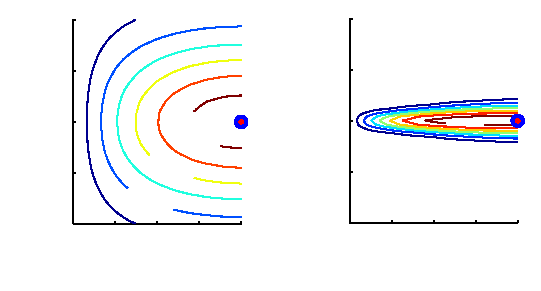
\includegraphics[width=\unitlength]{1dgrasp_result.pdf}}%
    \put(0.1151589,0.08992018){\makebox(0,0)[lb]{\smash{0.2}}}%
    \put(0.18217497,0.08992018){\makebox(0,0)[lb]{\smash{0.25}}}%
    \put(0.27003572,0.08992018){\makebox(0,0)[lb]{\smash{0.3}}}%
    \put(0.33673164,0.08992018){\makebox(0,0)[lb]{\smash{0.35}}}%
    \put(0.4249133,0.08992018){\makebox(0,0)[lb]{\smash{0.4}}}%
    \put(0.08972926,0.1171398){\makebox(0,0)[lb]{\smash{-0.5}}}%
    \put(0.07593948,0.20747584){\color[rgb]{0,0,0}\makebox(0,0)[lb]{\smash{-0.25}}}%
    \put(0.10355064,0.2982193){\makebox(0,0)[lb]{\smash{0}}}%
    \put(0.08669901,0.39782419){\makebox(0,0)[lb]{\smash{0.25}}}%
    \put(0.09666237,0.48644253){\makebox(0,0)[lb]{\smash{0.5}}}%
    \put(0.23790599,0.1699559){\rotatebox{-22.99998994}{\makebox(0,0)[lb]{\smash{0.04}}}}%
    \put(0.27574288,0.23088155){\rotatebox{-25.9999936}{\makebox(0,0)[lb]{\smash{0.08}}}}%
    \put(0.33923275,0.31457275){\rotatebox{-51.0000188}{\makebox(0,0)[lb]{\smash{0.12}}}}%
    \put(0.01695468,0.30375214){\color[rgb]{0,0,0}\makebox(0,0)[lb]{\smash{$u_2$}}}%
    \put(0.27728722,0.04517519){\color[rgb]{0,0,0}\makebox(0,0)[lb]{\smash{$u_1$}}}%
    \put(0.61970258,0.09198088){\makebox(0,0)[lb]{\smash{0.2}}}%
    \put(0.68671864,0.09198088){\makebox(0,0)[lb]{\smash{0.25}}}%
    \put(0.77457939,0.09198088){\makebox(0,0)[lb]{\smash{0.3}}}%
    \put(0.84127531,0.09198088){\makebox(0,0)[lb]{\smash{0.35}}}%
    \put(0.92945698,0.09198088){\makebox(0,0)[lb]{\smash{0.4}}}%
    \put(0.83165564,0.29547016){\rotatebox{-3.00000411}{\makebox(0,0)[lb]{\smash{0.7}}}}%
    \put(0.52418668,0.30637183){\color[rgb]{0,0,0}\makebox(0,0)[lb]{\smash{$u_2$}}}%
    \put(0.7845194,0.05087321){\color[rgb]{0,0,0}\makebox(0,0)[lb]{\smash{$u_1$}}}%
    \put(0.26204153,0.00490434){\color[rgb]{0,0,0}\makebox(0,0)[lb]{\smash{(a)}}}%
    \put(0.79104124,0.0040583){\color[rgb]{0,0,0}\makebox(0,0)[lb]{\smash{(b)}}}%
    \put(0.58730417,0.21390265){\color[rgb]{0,0,0}\makebox(0,0)[lb]{\smash{-0.25}}}%
    \put(0.59889533,0.11916901){\makebox(0,0)[lb]{\smash{-0.5}}}%
    \put(0.61271672,0.30024851){\makebox(0,0)[lb]{\smash{0}}}%
    \put(0.59586509,0.3998534){\makebox(0,0)[lb]{\smash{0.25}}}%
    \put(0.60582844,0.48847175){\makebox(0,0)[lb]{\smash{0.5}}}%
  \end{picture}%
\endgroup%
